\documentclass[10pt]{article}
\usepackage{../EllioStyle}
\usepackage{listings}
\usepackage{multicol}

\definecolor{codegreen}{rgb}{0,0.6,0}
\definecolor{codegray}{rgb}{0.5,0.5,0.5}
\definecolor{codepurple}{rgb}{0.58,0,0.82}
\definecolor{backcolour}{rgb}{0.95,0.95,0.92}

\usepackage[small]{titlesec}

\lstdefinestyle{mystyle}{
%    backgroundcolor=\color{backcolour},   
    commentstyle=\color{codegreen},
    keywordstyle=\color{magenta},
    numberstyle=\tiny\color{codegray},
    stringstyle=\color{codepurple},
    basicstyle=\ttfamily\footnotesize,
    breakatwhitespace=false,         
    breaklines=true,                 
    captionpos=b,                    
    keepspaces=true,                 
    numbers=left,                    
    numbersep=5pt,                  
    showspaces=false,                
    showstringspaces=false,
    showtabs=false,                  
    tabsize=2
}

\titlespacing{\section}{0pt}{0pt}{0pt}
\setlength{\parskip}{8pt}

\title{Notesheet}
\author{Elliott Pryor}
\date{October 7 2021}

\rhead{Notesheet for Exam 1}

\begin{document}
\multicols{2}

\section{Biology}

DNA - ATCG - Written 5' to 3'. 
Humans have 3G base pairs, 23 chromosome, avg gene is about 1K-2Kbp

RNA - UAGC - Single stranded. 
Introns are bits that ultimately get cut out of mRNA, begins with AG ends with GT.


Central Dogma - Transcription: DNA $\rightarrow$ RNA,
Translation: RNA $\rightarrow$ protein,
Post Translation Modification: clean up protein

\begin{figure}[H]
    \centering
    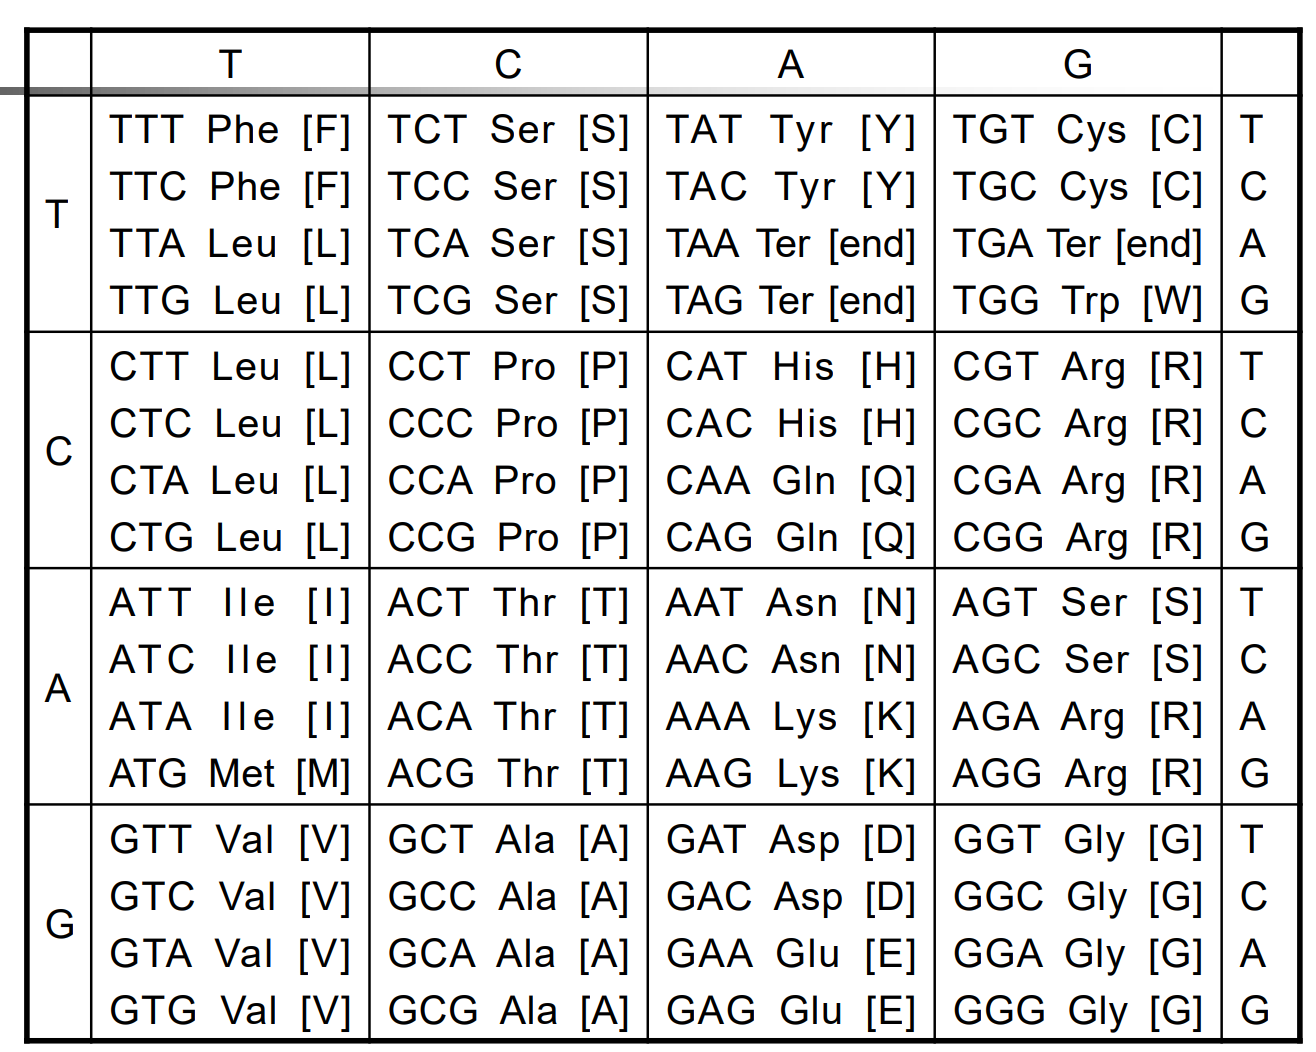
\includegraphics[width=0.7\linewidth]{proteins.png}
    \label{fig:proteins}
\end{figure}

SNP - single nucleotide polymorphism - ie. mutation.

Tools - Restriction Enzymes: EcoRi digests protein and breaks it at a specific point. 
Adds sticky ends - Shotgun: randomly break DNA - PCR: polymerase chain reaction.
- DNA Array: put specific target sequence in a cell, if DNA has it it reacts so it is a way to see if DNA has genes.


\section{Z-Algorithm}
Solves exact pattern matching algorithm.

\begin{algorithm}[H]
    \begin{algorithmic}[1]
    %\algsetup{linenosize=\tiny}
    \tiny
    \Function{Z-Algorithm}{$S$}
    
        \State l, r = 0
        \For{k = 2 .. n}
            \If{k > r}
                \State find $z_k$ by comparing S[k .. n] and S[1 .. n]
                \State If $z_k > 0$, $r = k + z_k - 1$, $l = k$
            \Else
                \State $k' = k - l + 1$
                \State $\beta = r - k + 1$
                \State If $z_{k'} < \beta$: $z_k = z_{k'}$
                \If {$z_k' \geq \beta$}
                    \State compare $S[\beta + 1 .. n]$ with $S[r+1 .. n]$ until mismatch at $q \geq r + 1$
                    \State $z_k = q-k$
                    \State $l = k$
                    \State $r = q-1$
                \EndIf
            \EndIf
        \EndFor

    \State \textbf{return} Z
    
    \EndFunction
    \end{algorithmic}
\end{algorithm}

This solves prefix matching problem returns an array of the matches.
For exact pattern matching do $S + \$ + T$ and return locations where score $= |S|$ after the \$ position.
This runs in $O(n)$ time, or $O(|S| + |T|)$ time for the exact pattern matching problem.

\section{Y-Algorithm}
Solves multiset matching problem. 
Goal is to check if all the letters in a pattern appear consecutively, without regard to order.
The intuition of the program is to initialize C to store counts of each letter in pattern.
Then we slide a window along and adjust counts.
We track a left and right end of the box of matches found so far in order to reduce redundant checks.
If all the counts are 0, then we have a match.
This runs in $O(n)$ time


\section{Global Alignment}
The goal is to find the optimal alignment of two strings.
This can be edit distance: where $\delta(x, x) = 0$, $\delta(x, y) = -1$
Which essentially counts the number of differences in the string. Or it can be a more complicated metric.
The global alignment score problem has $\delta(x, x) = 2$, $\delta(x,y) = -1$
Running time is $O(nm)$
\begin{algorithm}[H]
    \begin{algorithmic}[1]
    %\algsetup{linenosize=\tiny}
    \tiny
    \Function{Needleman-Wunch}{$S, T$}
        \State V = n x m matrix.
        \State $V[0,0] = 0$, $V[0,j] = V[0,j-1] + \delta(\_, T[j])$, $V[i,0] = V[i-1,0] + \delta(S[i], \_)$
        \State Loop over rows/cols
        \State $V[i,j] = max \begin{cases}
            V[i-1, j-1] + \delta(S[i], T[j]) \\
            V[i-1, j] + \delta(S[i], \_) \\
            V[i, j-1] + \delta(\_, T[j])
        \end{cases}$

    \State \textbf{return} $V[n, m]$
    \EndFunction
    \end{algorithmic}
\end{algorithm}

\begin{figure}[H] 
    \centering
    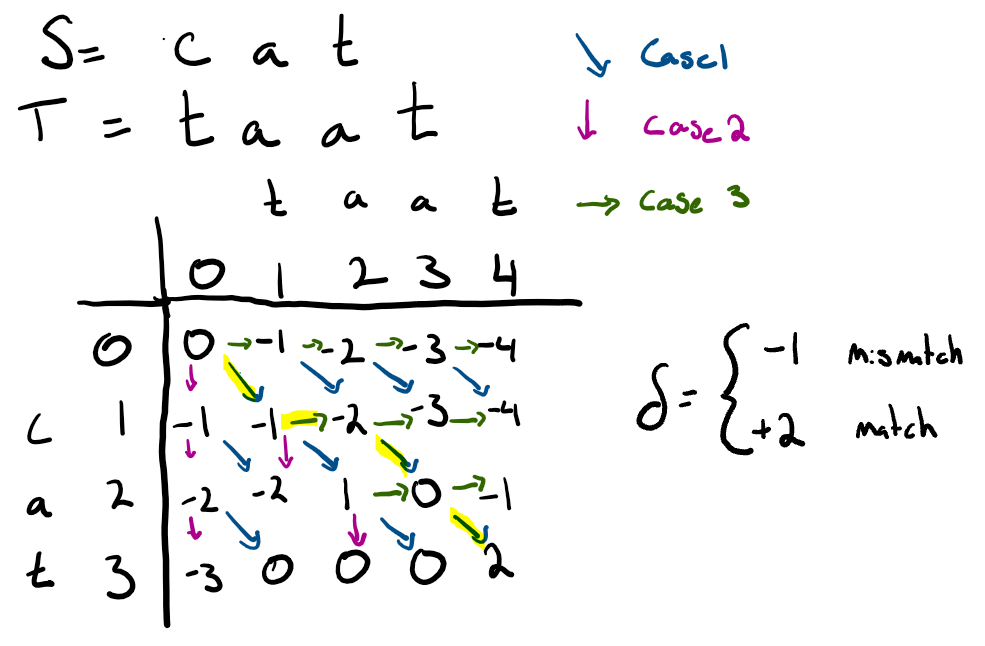
\includegraphics[width=0.7 \linewidth]{global_alignment.png}
    \label{fig:}
\end{figure}

\subsection{Four Russians Speedup}
Four Russians does same as Needleman Wunsch. But computes in t x t blocks.
The idea is to compute just the perimeter of the block. 
Optimal value of $t = \frac{\log_{3 |\Sigma|}n}{2}$.
Edit distance can be computed in $O(n^2 / \log n)$

\section{Local Alignment}
Goal is to find optimal alignment of any substrings within the words.
This is Smith-Waterman algorithm. It is almost identical to the Needleman Wunsch,
but with a case 0 added. $V[i,j] = max \begin{cases}
    0 \\
    V[i-1, j-1] + \delta(S[i], T[j]) \\
    V[i-1, j] + \delta(S[i], \_) \\
    V[i, j-1] + \delta(\_, T[j])
\end{cases}$ 

\section{Suffix Trees}
Build a trie with all the possible suffix's of an input.
Typically append an extra special character to the end \$ to mark the end of a string.
This can be used in a generalized suffix tree to identify which bits belong to which input based on unique end character.
To save space, store the letters as index slices into the string instead of raw characters.
Naiive way to build takes $O(n^2)$, but can be done in $O(n)$ .
\begin{figure}[H] 
    \centering
    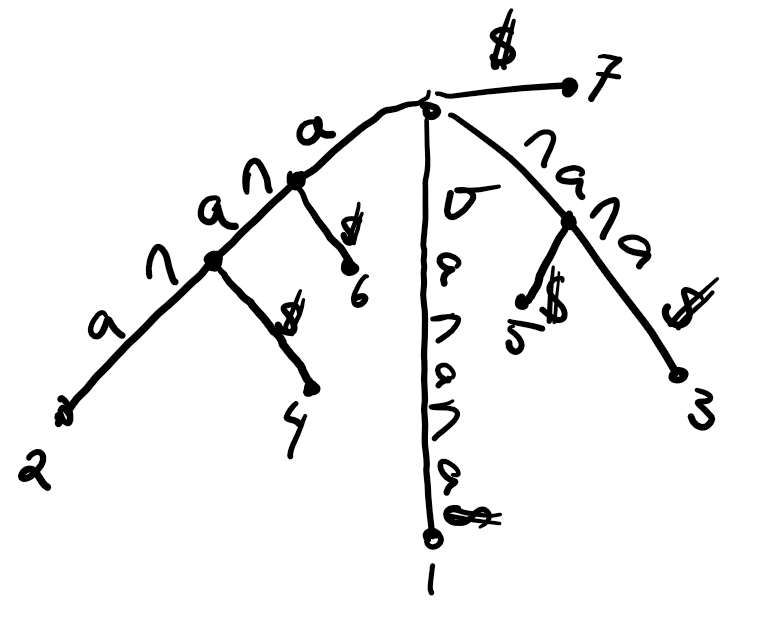
\includegraphics[width=0.7 \linewidth]{suffix_tree.png}
\end{figure}


Exact pattern matching queries can be done quite fast $O(m + \# occ)$.
Just follow pattern down suffix tree. Return number of nodes below the pattern.

Longest common substring. Use a generalized suffix tree (put both S and T in).
Use DFS to label height of internal nodes, and to label which strings can be reached from the node.
Longest common substring is the depth of deepest internal node from which both strings are reachable. 

Longest common prefix. Similar concept as LCS. LCP(i, j) = LCP of $S[i .. n]$ and $S[j .. n]$.
So find leaf nodes corresponding to $i, j$. Then LCP is the depth of lowest common ancestor.
(lowest internal node from which node i and j can be reached)

Palindrome algorithm. Kind of complicated. Goal is to find longest palindrom centered around $i$ for all $i$.
Build generalized suffix tree for $S, S^{rev}$. Find depth of all internal nodes.
Build magic datastructure that allows constant time lookup to compute Lowest Common Ancestor (LCA) (this is for LCP computations)
For even palindromes: Compute $k = LCP(S_i, S^{rev}_{n-i+2})$, report $S[i-k .. i + k - 1]$. 
For odd palindromes: Compute $k = LCP(S_i, S^{rev}_{n-i+1})$, report $S[i-k + 1 .. i + k - 1]$. 

\section{Suffix Array}
Create all suffix of string S. Sort by lexicographical order.
At $i^{th}$ spot in the array, put the start position of the $i^{th}$ suffix in lexicographical order. 


\end{document}